\documentclass[12pt,letterpaper]{article}

%Packages
\usepackage{xcolor}
\usepackage{changepage}
\usepackage{pdflscape}
\usepackage{fixltx2e}
\usepackage{textcomp}
\usepackage{fullpage}
\usepackage{natbib}
\usepackage{float}
\usepackage{latexsym}
\usepackage{url}
\usepackage{epsfig}
\usepackage{graphicx}
\usepackage{amssymb}
\usepackage{amsmath}
\usepackage{bm}
\usepackage{array}
\usepackage[version=3]{mhchem}
\usepackage{ifthen}
\usepackage{caption}
\usepackage{hyperref}
\usepackage{amsthm}
\usepackage{amstext}
\usepackage{enumerate}
\usepackage[osf]{mathpazo}
\usepackage{dcolumn}
\usepackage{lineno}
\usepackage{longtable}
\pagenumbering{arabic}


%Pagination style and stuff
\linespread{2}
\raggedright
\setlength{\parindent}{0.5in}
%\setcounter{secnumdepth}{0} 

\renewcommand\thefigure{A.\arabic{figure}}

\begin{document}

\section{Appendix A: Tree Inference}

\subsection{Morphological character states}
To obtain a realistic value for the probability of having \textit{k} characters states for each simulated morphological character, we randomly selected 100 morphological matrices, each with more than 100 characters each, from TreeBASE (\url{http://treebase.org/}). We only selected matrices published between 1985 and 2013 and covering 19 taxonomic classes (Chordata, Arthropoda, Annelida, Angiosperm, Gymnosperm and Pteridophyta). This resulted in a total of 22563 characters that had between two and 10 character states. We then extracted the proportion of characters with each number of states (two to 10) to give us an empirical estimate of the average number of character states for each character, as shown in Figure \ref{Fig_AppendixCharacters}. Most characters have two or three states, therefore we only simulate characters with two or three states, and sample these in proportion to their occurrence in our empirical data (probability of 0.85 for two states characters and 0.15 for three state characters). The code used for this section is available at \url{https://github.com/TGuillerme/Total_Evidence_Method-Missing_data/blob/master/Analysis/MorphologicalCharacterStates.R}.

\begin{figure}
\centering
\includegraphics[keepaspectratio=true]{SupplementaryFigures/TEM_Fig-AppendixCharacters.pdf}
\caption{The proportion of morphological characters with between two and 10 character states extracted from 100 randomly selected empirical matrices downloaded from TreeBASE.}
\label{Fig_AppendixCharacters}
\end{figure}

\subsection{Morphological rates estimations results}
To test the sensitivity of the Bayesian prior on the morphological rates distribution shape ($\alpha$ = 0.5), we compared the shape of the distribution of our generated morphological characters ($\alpha_{TRUE}$) to the shape of the distribution of morphological characters rate estimated by the Bayesian inference ($\alpha_{EST}$).
The $\alpha_{TRUE}$ parameter was estimated by fitting a gamma distribution to the 100 individual morphological rates (randomly sampled from a gamma distribution with $\alpha$ = 0.5) using the \texttt{fitdistr} function from the \texttt{MASS R} package \citep{MASS}.
We measured the difference as:
\begin{equation}
\Delta\alpha=\alpha_{EST} - \alpha_{TRUE}
\end{equation}
We then calculated the mode and the 95\% and 50\% confidence intervals over the 50 chains using the \texttt{hdr} function from the \texttt{hdrcde R} package \citep{hdrcde}.
The code used for this section is available at \url{https://github.com/TGuillerme/Total_Evidence_Method-Missing_data/blob/master/Analysis/Rates_estimates.R}.

\begin{figure}
\centering
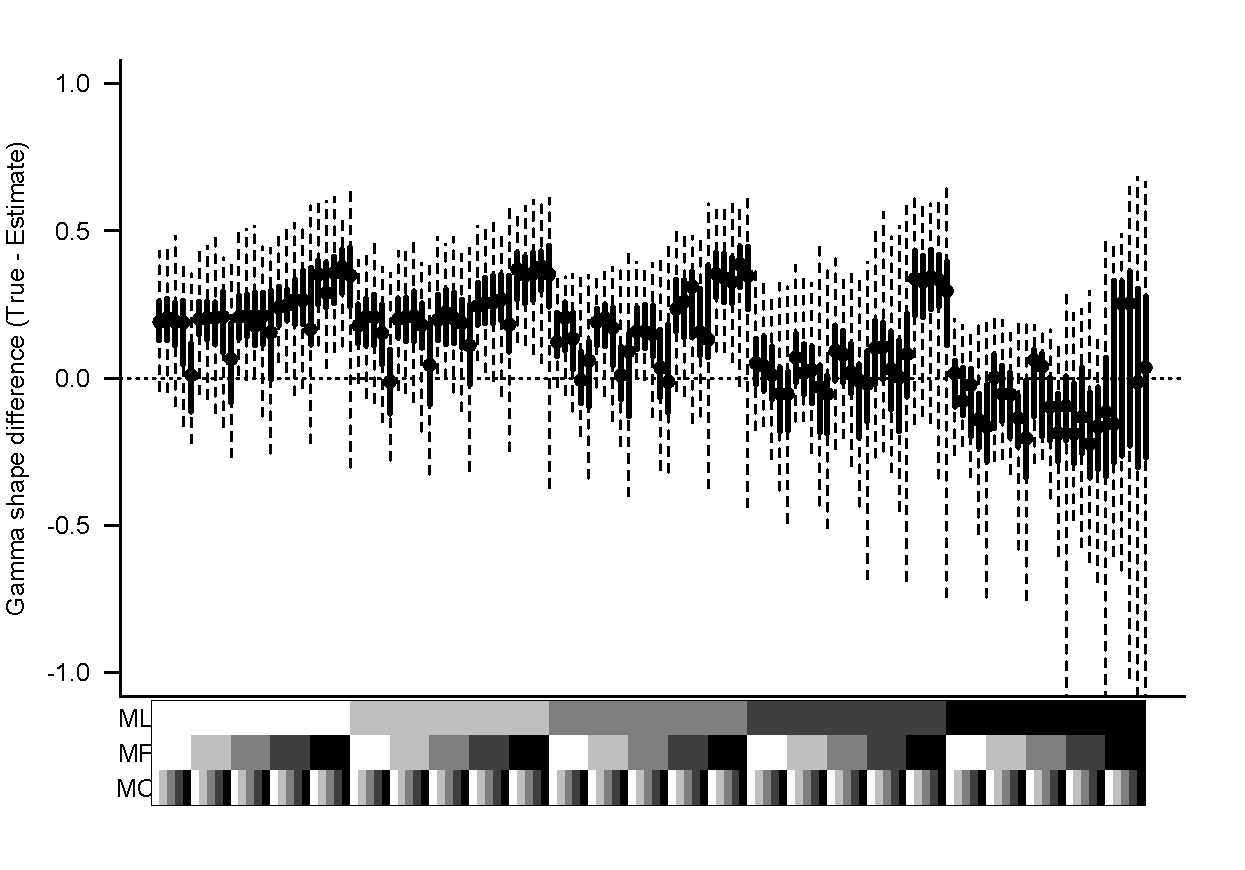
\includegraphics[width=\textwidth,keepaspectratio]{SupplementaryFigures/Rates_estimates.pdf}
\caption{Differences between the simulated rate of each morphological character ($\alpha$ parameter) and the Bayesian estimates for the trees with missing data. The x axis shows the percentage of missing data from 0\% (white) to 75\% (black) for the two parameters: $M_{L}$ (upper line), $M_{F}$ (middle line) and number of characters from 100 to 25 for the parameter $N_{C}$ (lower line). Positive values shows overestimation of the parameter and negative values shows underestimation. One unit of difference means that the estimated rate is twice as big/small than the true rate. The graph shows the modal value (points), and the 50\% (thick solid lines) and 95\% (thin dashed lines) confidence intervals of the distributions of the rates estimates.}
\label{Fig_AppendixCharacters}
\end{figure}

\subsection{Effect of the starting tree in Bayesian inference}
We used the ``true'' tree as a starting tree for the two MCMC chains in the Bayesian inference for decreasing the computing time.
To assess if this had an effect on the topology of the ``best'' tree, we ran a sub-sample of trees using a different random tree for the two MCMC chains \citep[default MrBayes option;][]{Ronquist2012mrbayes}.
We tested this effect on five trees with the five levels of missing data (i.e. first tree: $M_L$=0\%, $M_F$=0\% and $N_C$=100; second tree: $M_L$=10\%, $M_F$=10\% and $N_C$=90, etc.) on the first 20 simulation chains.
We then compared the trees inferred using the ``true'' tree as a starting tree to the trees using a random tree as a starting tree using the normalised Robinson-Foulds and Triplets metrics.
Additionally, we compared the trees inferred using a random tree as a starting tree to the ``best'' tree (inferred using the ``true'' tree as a starting tree) and to the ``true'' tree to see whether our results varied if we didn't used the ``true'' tree as a starting tree.

\begin{table}[!ht]
\caption{Normalised topological metric between trees using the ``true'' or a random tree as a starting tree for the MCMC chains.}
\centering
\begin{tabular}{|l|c|c|c|c|c|c|c|}
  \hline
 Tree &  Metric & Min. & 1st Qu. & Median & Mean & 3rd Qu. & Max. \\ 
  \hline
    $M_L$=0\%; $M_F$=0\%; $N_C$=0\%          & $RF$ & 0.00 & 0.00 & 0.10 & 0.20 & 0.32 & 1.00 \\ 
                                             & $Tr$ & 0.34 & 0.49 & 0.61 & 0.62 & 0.75 & 1.00 \\ 
    $M_L$=10\%; $M_F$=10\%; $N_C$=10\%       & $RF$ & 0.03 & 0.54 & 0.69 & 0.64 & 0.77 & 0.98 \\ 
                                             & $Tr$ & 0.08 & 0.57 & 0.65 & 0.64 & 0.73 & 0.82 \\ 
    $M_L$=25\%; $M_F$=25\%; $N_C$=25\%       & $RF$ & 0.02 & 0.74 & 0.80 & 0.79 & 0.89 & 0.98 \\ 
                                             & $Tr$ & 0.21 & 0.67 & 0.73 & 0.72 & 0.77 & 0.84 \\ 
    $M_L$=50\%; $M_F$=50\%; $N_C$=50\%       & $RF$ & 0.00 & 0.00 & \textbf{0.00} & \textbf{0.01} & 0.01 & 0.04 \\ 
                                             & $Tr$ & 0.08 & 0.38 & 0.59 & 0.57 & 0.73 & 0.84 \\ 
    $M_L$=75\%; $M_F$=75\%; $N_C$=75\%       & $RF$ & 0.00 & 0.00 & \textbf{0.01} & \textbf{0.02} & 0.04 & 0.11 \\ 
                                             & $Tr$ & 0.21 & 0.36 & 0.56 & 0.55 & 0.74 & 0.87 \\ 
   \hline
\end{tabular}
\label{Tab_Results-Difference_methods}
\end{table}

%Incl table + incl figure 



\newpage
\subsection{Tree Inference Software settings}

For clarity we have provided the exact settings used in our tree building below.

\subsubsection{Maximum Likelihood: RAxML version 8.0.20 \cite{Stamatakis21012014}}

\begin{itemize}
  \item Molecular data: GTR + $\Gamma_4$ (-m GTRGAMMA)
  \item Morphological data: M\textit{kv} + $\Gamma_4$ (-K MK)
  \item Support: Rapid Boostrap algorithm (LSR), 1000 replicates
\end{itemize}

\subsubsection{Bayesian: MrBayes version 3.2.1 \cite{Ronquist2012mrbayes}}

\begin{itemize}
  \item Priors: Molecular data
  \begin{itemize}
    \item Rates distribution shape ($\alpha$) = 0.5
    \item Transition/Transversion ratio = 2 ($\beta$(80,40))
    \item Starting tree: "True" tree topology with each branch length = 1
  \end{itemize}
  \item Priors: Morphological data
  \begin{itemize}
    \item rates distribution shape ($\alpha$) = 0.5
  \end{itemize}
  \item Models
  \begin{itemize}
    \item Molecular data: HKY + $\Gamma_4$
    \item Morphological data: M\textit{kv} + $\Gamma_4$
  \end{itemize}
  \item MCMC
  \begin{itemize}
    \item Two runs
    \item Four chains per run
    \item Generations $<$ 5$\times$$10^7$
    \item Sample frequency = 1.05$\times$$10^4$
    \item ASDS diagnosis frequency = 5$\times$$1^4$
    \item ASDS $<$ 0.01
    \item ESS $>>$ 200
    \item Burnin = 25\%
  \end{itemize}
\end{itemize}

\bibliographystyle{sysbio}
\bibliography{Supp_Ref}

%END
\end{document}